%%%%%%%%%%%%%%%%%%%%%%%%%%%%%%%%%%%%%%%%%%%%%%%%%%%%%%%%%%%%%%%%%%%%%%%%%%%%%%%%
%2345678901234567890123456789012345678901234567890123456789012345678901234567890
%        1         2         3         4         5         6         7         8

%\documentclass[letterpaper, 10 pt, conference]{ieeeconf}  % Comment this line out
                                                          % if you need a4paper
\documentclass[a4paper, 10pt, conference]{ieeeconf}      % Use this line for a4
                                                          % paper

\IEEEoverridecommandlockouts                              % This command is only
                                                          % needed if you want to
                                                          % use the \thanks command
\overrideIEEEmargins
% See the \addtolength command later in the file to balance the column lengths
% on the last page of the document



% The following packages can be found on http:\\www.ctan.org
%\usepackage{graphics} % for pdf, bitmapped graphics files
%\usepackage{epsfig} % for postscript graphics files
%\usepackage{mathptmx} % assumes new font selection scheme installed
%\usepackage{times} % assumes new font selection scheme installed
%\usepackage{amsmath} % assumes amsmath package installed
%\usepackage{amssymb}  % assumes amsmath package installed
\usepackage[T1]{fontenc}
\usepackage[latin1]{inputenc}
\usepackage{graphicx}

\title{\LARGE \bf
A flexible visual framework for debugging complex robotic systems
}

%\author{ \parbox{3 in}{\centering Huibert Kwakernaak*
%         \thanks{*Use the $\backslash$thanks command to put information here}\\
%         Faculty of Electrical Engineering, Mathematics and Computer Science\\
%         University of Twente\\
%         7500 AE Enschede, The Netherlands\\
%         {\tt\small h.kwakernaak@autsubmit.com}}
%         \hspace*{ 0.5 in}
%         \parbox{3 in}{ \centering Pradeep Misra**
%         \thanks{**The footnote marks may be inserted manually}\\
%        Department of Electrical Engineering \\
%         Wright State University\\
%         Dayton, OH 45435, USA\\
%         {\tt\small pmisra@cs.wright.edu}}
%}

\author{Felix Kaser$^{1}$, Bruce MacDonald (?)$^{2}$% <-this % stops a space
%\thanks{*This work was not supported by any organization}% <-this % stops a space
\thanks{$^{1}$F. Kaser is with ...? Universit�t Augsburg, TU M�nchen, LMU M�nchen, University of Auckland
        {\tt\small kaserf at in.tum.de}}%
\thanks{$^{2}$B. MacDonald is with the Department of Electrical Engineering, University of Auckland,
        New Zealand
        {\tt\small b.macdonald at auckland.ac.nz}}%
}


\begin{document}



\maketitle
\thispagestyle{empty}
\pagestyle{empty}


%%%%%%%%%%%%%%%%%%%%%%%%%%%%%%%%%%%%%%%%%%%%%%%%%%%%%%%%%%%%%%%%%%%%%%%%%%%%%%%%
\begin{abstract}

The abstract is still empty

\end{abstract}


%%%%%%%%%%%%%%%%%%%%%%%%%%%%%%%%%%%%%%%%%%%%%%%%%%%%%%%%%%%%%%%%%%%%%%%%%%%%%%%%
\section{INTRODUCTION}

\begin{itemize}[Introduction:]

\item initial approach to integrate tracepoints?
\item different approach to debug
\item making printf debugging better
\item current problems with robot debugging

\end{itemize}

Debugging complex robotic systems has proven to be more difficult then debugging normal (still complex) systems [check citation!] \cite{Collett2010}. One of the biggest problems when debugging robotic systems is the non-interruptible nature of robotic applications. Sometimes it is hard or even impossible to interrupt the execution of a robot without being a thread to the robot hardware and the persons and equipment in the environment where the robot is deployed. For example you can not just interrupt a quad-copter in mid-flight to step through the algorithm to find a bug. [citation?]

One approach to address this issue is to keep two separated controllers: a low level controller that keeps the essential parts of the robot running (e.g. keep the quad-copter flying) and a high level controller that runs the application logic code which is debugged. This only solves part of the problem because developing the low level controller is still not interruptible. [citation?]

Another approach has come up in the past and it is more thorough, the concept of tracepoints is used to debug a robot application without interrupting the execution but analysing the trace post-mortem (and more recently also viewing the results live \cite{Gumbley2009}. Using tracepoints to debug a program is a highly instrumented way of debugging and does not require a modification of the source code. However the tracepoints approach is quite complex and pre-execution configuration takes a substantial effort and skill, which many developers won't like to take upon them. [badly written, rewrite, no proof]

[write a paragraph about AR debugging?]

In the end many developers fall back to printf-debugging because it is something the can do with the skills they already have without learning a new toolset and setting up a tracing or debugging process [proof?]. One major downside of printf-debugging is the text-only representation of data. The developer tries to understand what the program is doing by looking at endless streams of data in a console and tries to make sense of the data. In this paper we [we or I?] present a new approach to improve printf-debugging. A framework was developed to add type information to prinft-like-statements which can be used to display data-type specific widgets on a dashboard that visualize the debugged data in a more natural way. The developer can choose which visualization he prefers and suits his mental model of the data best. [unnecessary?: While printf-debugging has its downsides, there are also benefits to printf-debugging. The developer knows exactly where the printf-statements are and this makes it easy to understand the flow of a program.]

\section{RELATED WORK}

\begin{itemize}[Related work:]

\item ROS
\item LabView
\item tracepoints?

\end{itemize}

\subsection{ROS - Robot Operating System}
[this subsection should be shorter]

The Robot Operating System (ROS) is an Open Source framework for complex robotic systems. The first work on ROS was done as part of the STanford Artificial Intelligence Robot (STAIR) in 2007 \cite{Quigley2007}. The original software library was called \emph{Switchyard} and had been developed at Stanford. Later the library was refined and generalized to also suit the requirements of the Personal Robot Program at Willow Garage\footnote{www.willowgarage.com} \cite{Quigley2009}. The resulting general framework has been released as Open Source \cite{Quigley2009} and this section gives a short overview over the most important principles in ROS.

ROS was built to abstract from the hardware of the robot and create modular robot software, which can run on different robots and on different machines. This makes it easier to write software for robots and distribute the work to different teams, each team focusing on one part of the robot. The modules in ROS are called nodes and several nodes executed together are called a stack. ROS packages bundle nodes and stacks and are used to make software modules available to other developers. Everyone can create their own package which can be indexed by ROS so that your software modules can be found, downloaded and used by other developers. There exist many packages, nodes and stacks for some of the most common problems in robotics (e.g. navigation, localization, joint movement, etc.) and can easily be re-used.

The communication between ROS nodes can be done asynchronously through a publish/subscribe mechanism and synchronously through services. Nodes can send messages by publishing a message on a topic and receive messages by subscribing to that topic. This mechanism is really flexible and decouples the sender from the receiver. A publisher node does not need to know if there are other nodes listening and vice versa. For synchronous communication and guaranteed delivery of messages, services can be invoked. The routing is established during runtime through the ROS core. The core of ROS was kept really slim and only contains the most essential parts of the framework (such as the inter node communication). ROS can run on several machines distributed in a network, the only restriction is that every node needs to know the address of the core (master node) in order to communicate with other nodes.

\subsection{LabView}

LabView has similar draggable widgets to make the development of systems easier.

\subsection{Tracepoints?}

Are tracepoints still that relevant to my work to list it here?

\section{ROSDASHBOARD}

Design, approach, integration, ROS philosophy...

\begin{itemize}

\item design (requirements)
\item approach
\item integration
\item ROS philosophy

\end{itemize}

\subsection{Overview}
ROSDashboard is a new tool in the ROS environment. It is built to allow developers easy visualization of data streams. It is built around a central dashboard where developers can add visualization widgets with drag and drop from a toolbox. Currently there are only the most basic widgets implemented to visualize data. In future there should be added more and more widgets. This effort could come from the robot developers themselves through a simple plugin mechanism. The developers know best what widgets they need to visualize their data.

\subsection{Requirements}
Requirements (easy to install and use, simple to extend, base tool for further development and evaluation)

\subsubsection{Openness}
One of the requirements is to be open. Open in terms of Open Source but also regarding the other requirements like extendibility and adaptability. Openness helps to spread the word and gain a higher user base faster. [citation?]
\subsubsection{Low configuration overhead}
The goal was to create a useful tool that is easy to use and can be used by anyone without much configuration, setup or learning overhead. This contributes to a high user acceptance and a low entrance barrier [better wording?] for new users.
\subsubsection{Extendibility and adaptability}
Different developers prefer to visualize their data differently and every project is different. It is important [why important?] to create a system that can be extended to be more powerful and adapted to different use cases. Especially in robotics where common standards are not yet defined and the variety of tools, frameworks and robot hardware is big.
\subsubsection{ROS philosophy [really?]}
ROS is designed to have a really small core with as many tools build around the common core as needed. The principle is to have small tools that do one thing but are really specialized and sophisticated. This philosophy is followed and encouraged by the ROS core developers. It is important to follow this principle to reach a high acceptance among the ROS community and to fit in as good as possible with other tools.


\subsection{Design}
ROS client libraries currently fully support Python and C++, client libraries for Java and other languages are currently under development. For ROSDashboard Python was chosen as the target language, because it is a good match for fast prototyping and iterative development. Python's duck typing [reference] turned out to be a big help for topic introspection (see implementation details \ref{topic introspection}). Qt is used for the graphical part of the tool which also reflects the general policy in the ROS community (before Qt wxWidgets was the graphical toolkit of choice).

Although the current software does not support third party widgets as plugins, the structure of the internal widgets is aligned to allow easy integration of such a feature in the near future. For now if a third party wants to have specialized widgets, it needs to modify the source code and add the code for widgets directly to the source tree.

ROSDashboard was released as Open Source from the very beginning to allow external contributions and feedback. The source code is hosted on Github \footnote{http://github.com/kaserf/rosdashboard}. A prototype was announced to the ROS community and valuable feedback was gathered and documented. One of the most valuable feedback was to make ROSDashboard more generic and allow to visualize topics that publish String messages which are parsed to get the data for the visualization. This would make it possible to use ROSDashboard with existing projects that already contain extensive logging (but in text form).

\subsection{Implementation details}
\subsubsection{Topic introspection}
\label{topic introspection}
ROS topics were originally not designed and developed as something the user or developer chooses graphically. Topics are usually set up in the code. ROSDashboard exposes the topic setup in a graphical user interface and this turned out to become a challenge since one of the requirements is to have a low configuration overhead (see requirements section [add reference]). Normally you have to select a topic name and a message data type. The data type can be one of the standard message types (wrapping the basic types like Float, Integer, String and Boolean) or a more complex message type. To access one data element of a message the "datafield" field was introduced in the graphical interface. Using Pythons duck typing and the rostopic module it was possible to avoid the complexity of dynamically binding message types during runtime and detect the message type automatically. If a topic is not yet published (and thus the message type is not defined yet) the call to rostopic blocks until the message type becomes known. To avoid blocking of the user interface a listener thread was implemented to wait until a topic (message type) becomes available. Avoiding to manually ask the user for a message type makes the configuration of widgets easier and faster for the user and also keeps the implementation simpler (no dynamic binding of message type classes during runtime).

[show screenshot of topic subscription dialog?]

\begin{figure}[thpb]
  \centering
  \framebox{
    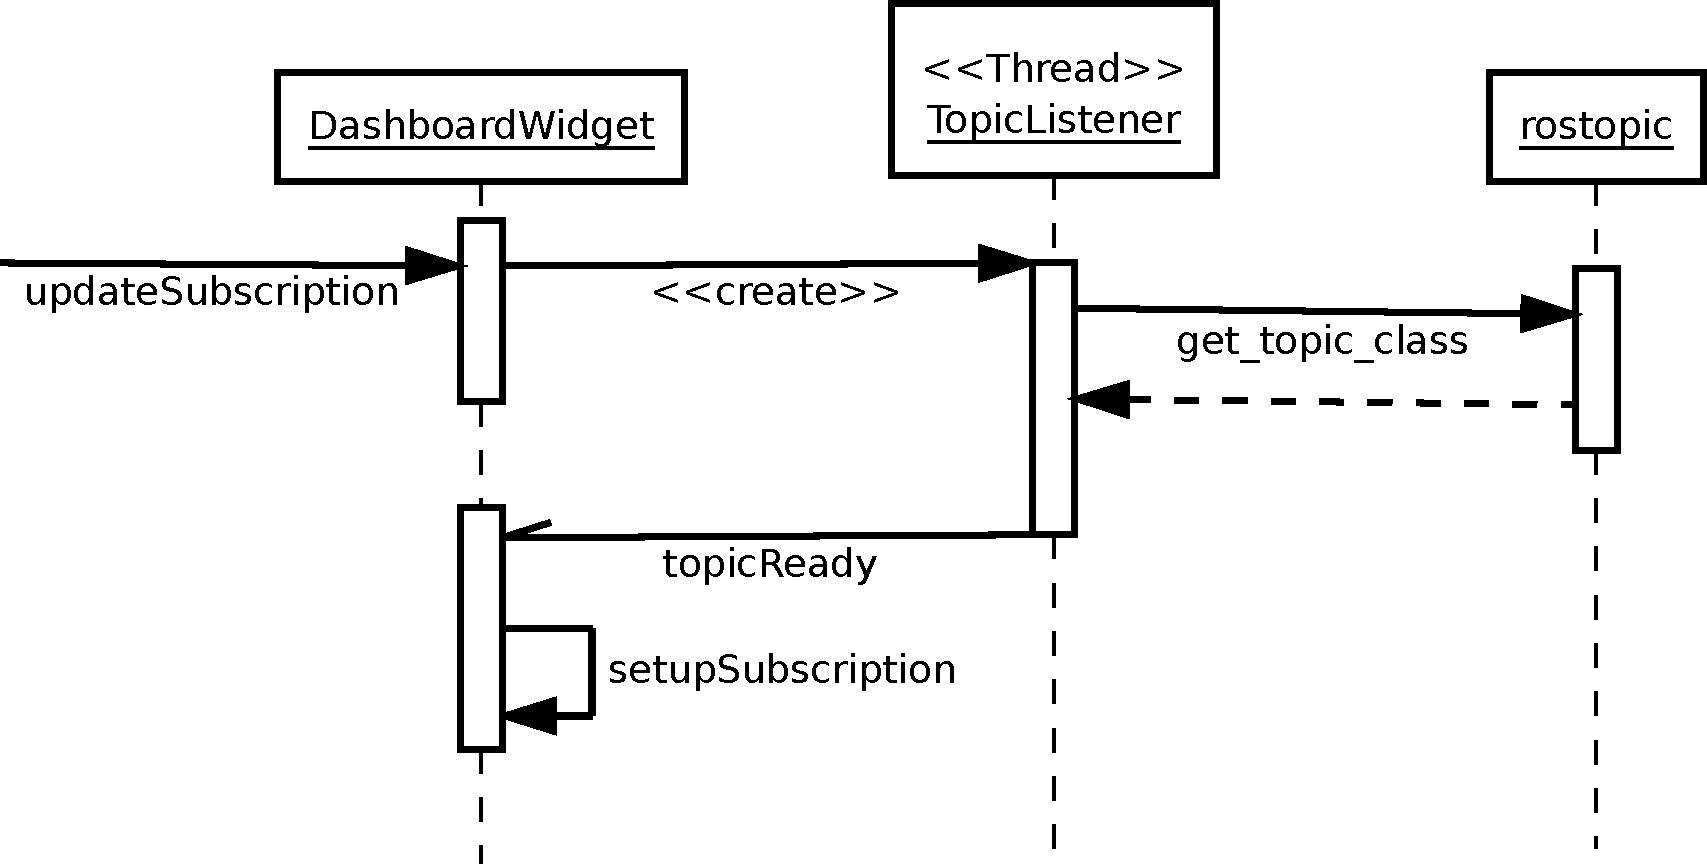
\includegraphics[scale=0.28]{diagrams/topic_subscription.pdf}
  }  
  \caption{Exemplary flow of events for updating the topic setting of a widget.}
  \label{topic subscription}
\end{figure}

\subsubsection{Object model}
The object model was designed to make it easy to extend ROSDashboard with more widgets. The abstract DashboardWidget class covers the general tasks that are the same for every widget. It provides hooks to overwrite some methods in the subclass if a widget needs to be more specific. This should allow easy integration of a plugin framework at [at? in? on?] a later stage, where third party widget developers only need to implement the specific parts of a new widget and the common tasks can be handled by the default implementation in DashboardWidget.

\begin{figure}[thpb]
  \centering
  \framebox{
    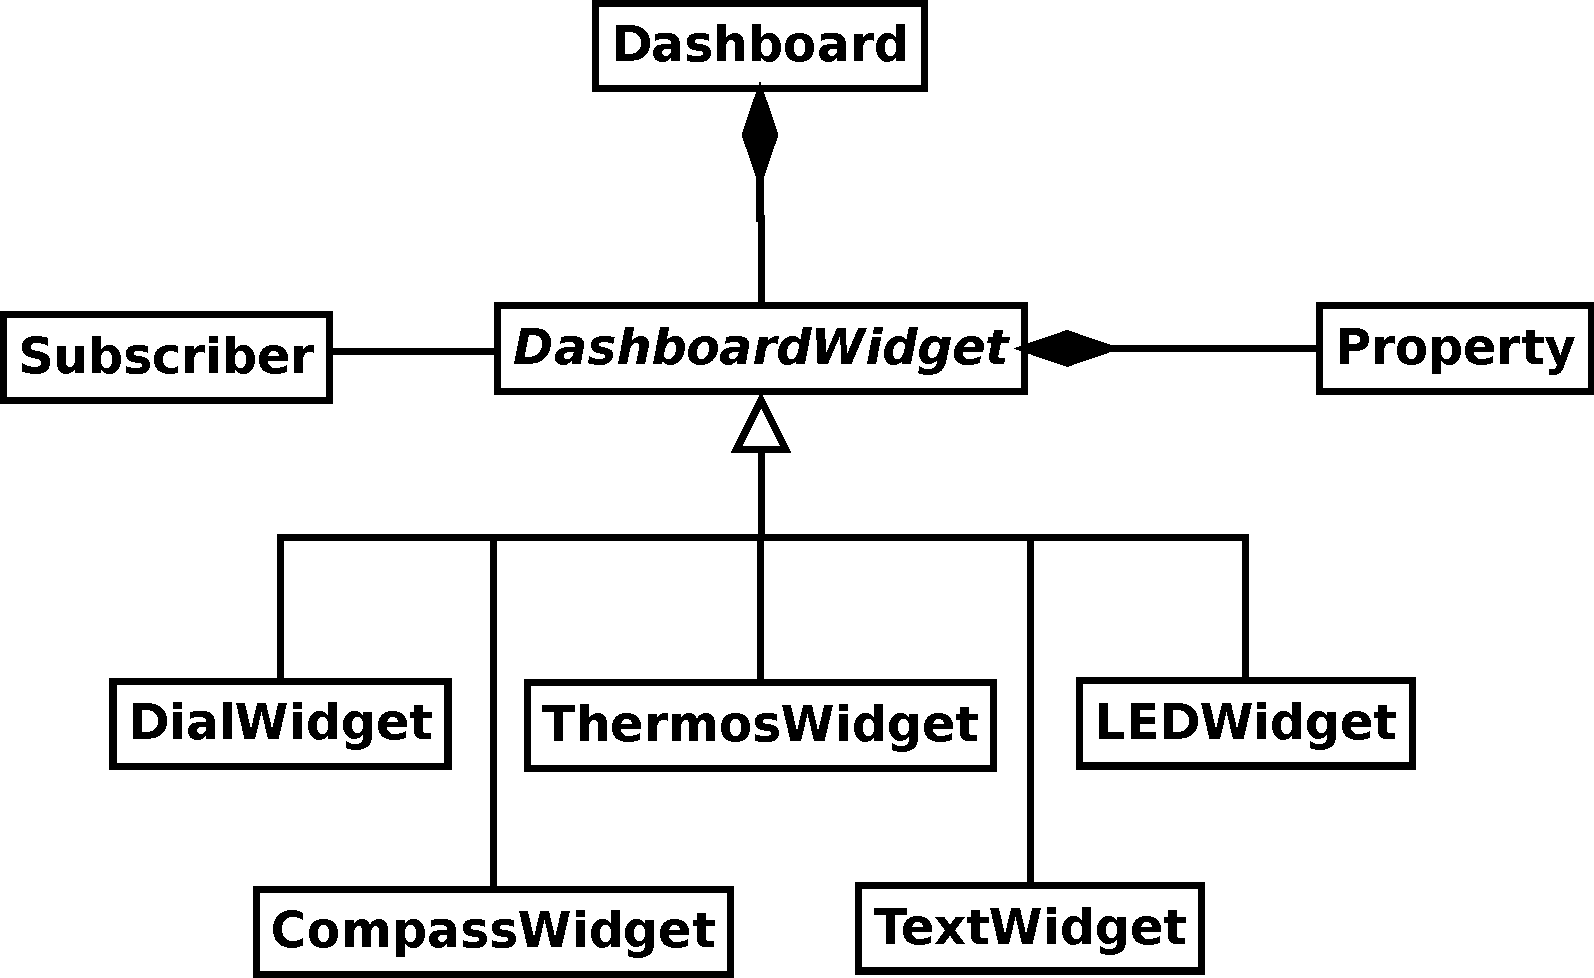
\includegraphics[scale=0.3]{diagrams/class_overview.pdf}
  }  
  \caption{Overview of the core object model structure.}
  \label{class overview}
\end{figure}

The subscription setup and the properties management was baked into DashboardWidget as well. This is mainly to keep these parts away from a plugin developer to make his life easier. The plugin developer only needs to specify which properties his widget needs and needs to implement the callback that gets called when the properties have been changed. DashboardWidget supports numeric, text and float properties. If more specific properties are needed the plugin can overwrite the whole properties part and not re-use the default implementation from DashboardWidget.

\subsection{Open Issues}
The next steps for ROSDashboard are to be integrated into RQT and a plugin framework to allow third parties to write widgets for ROSDashboard. A more long term plan for the project is to implement a parser that can extract data from text-based topics through regular expressions. Another long term plan is to generalize the widgets to have both subscription widgets and publisher widgets. One could have widgets that change settings of the robot and trigger special functions (a remote control for robots if you wish). [badly written, needs to be structured, extended and improved in general]

\section{THEORETICAL BACKGROUND}

This section probably is nonsense. I wanted to get into detail about the fast feedback loop, small changes to the code, how it affects the debugging and development style in general, small product increments, ...

\begin{table}[h]
\caption{An Example of a Table}
\label{table_example}
\begin{center}
\begin{tabular}{|c||c|}
\hline
One & Two\\
\hline
Three & Four\\
\hline
\end{tabular}
\end{center}
\end{table}

\section{FUTURE WORK}


\begin{itemize}

\item plugin structure
\item integrate into RQT
\item more widgets
\item widget designer (small python snippets?)
\item evaluation in real project

\end{itemize}

\section{CONCLUSIONS}

Do I need this section? What should I conclude about? Alternative approach to debugging? Fast feedback prototyping? (There was no evaluation so this section might be obsolete)

\addtolength{\textheight}{-12cm}   % This command serves to balance the column lengths
                                  % on the last page of the document manually. It shortens
                                  % the textheight of the last page by a suitable amount.
                                  % This command does not take effect until the next page
                                  % so it should come on the page before the last. Make
                                  % sure that you do not shorten the textheight too much.

%%%%%%%%%%%%%%%%%%%%%%%%%%%%%%%%%%%%%%%%%%%%%%%%%%%%%%%%%%%%%%%%%%%%%%%%%%%%%%%%



%%%%%%%%%%%%%%%%%%%%%%%%%%%%%%%%%%%%%%%%%%%%%%%%%%%%%%%%%%%%%%%%%%%%%%%%%%%%%%%%



%%%%%%%%%%%%%%%%%%%%%%%%%%%%%%%%%%%%%%%%%%%%%%%%%%%%%%%%%%%%%%%%%%%%%%%%%%%%%%%%

\section*{ACKNOWLEDGMENT}

Thank everyone :)


%%%%%%%%%%%%%%%%%%%%%%%%%%%%%%%%%%%%%%%%%%%%%%%%%%%%%%%%%%%%%%%%%%%%%%%%%%%%%%%%

%%%%% references %%%%%
\bibliographystyle{IEEEtranBST/IEEEtran}
\bibliography{bibtex/Master_Thesis}

\end{document}
